\documentclass[a4paper]{article}

\usepackage[paper=a4paper, left=1.5cm, right=1.5cm, bottom=1.5cm, top=3.5cm]{geometry}
\usepackage[spanish,activeacute]{babel}
\usepackage[utf8]{inputenc}
\usepackage{amsthm}
\usepackage{amsmath}
\usepackage{amsfonts}
\usepackage{amssymb}
\usepackage{alltt}
\usepackage{graphicx} %Para incluir el logo de la UBA
\usepackage{caratula} %Para armar el cuadro de integrantes
\usepackage{multirow} %Para poder poner varias lineas juntas sin divisiones en una tabla
\usepackage[lined,ruled,linesnumbered]{algorithm2e}
\usepackage{algpseudocode}
\usepackage{scrextend}
\usepackage{blindtext}

\usepackage{pdfpages}


%Cosas para escribir codigo fuente
%Fuente: http://en.wikibooks.org/wiki/LaTeX/Source_Code_Listings
\usepackage{listings}
\usepackage{color}

\setcounter{secnumdepth}{5}

\definecolor{mygreen}{rgb}{0,0.6,0}
\definecolor{mygray}{rgb}{0.5,0.5,0.5}
\definecolor{myorange}{rgb}{1,0.4,0.2}
\definecolor{myblue}{rgb}{0,0,0.65}


\makeatletter
\newcommand\invisiblesubsection[1]{%
  \refstepcounter{subsection}%
  \addcontentsline{toc}{subsection}{\protect\numberline{\thesubsection}#1}%
  \subsectionmark{#1}\phantom{}}
\makeatother

\newcommand{\insertfigscaled}[2]{
	\begin{figure}[!ht]
	\centering
	\includegraphics[width=#2]{#1}
	\end{figure}
}


%Configuracion para los listings
\lstset{ %
  backgroundcolor=\color{white},   % choose the background color; you must add \usepackage{color} or \usepackage{xcolor}
  basicstyle=\small,        % the size of the fonts that are used for the code
  breakatwhitespace=false,         % sets if automatic breaks should only happen at whitespace
  breaklines=true,                 % sets automatic line breaking
  captionpos=b,                    % sets the caption-position to bottom
  commentstyle=\color{mygreen},    % comment style
  deletekeywords={...},            % if you want to delete keywords from the given language
  escapeinside={\%*}{*)},          % if you want to add LaTeX within your code
  extendedchars=true,              % lets you use non-ASCII characters; for 8-bits encodings only, does not work with UTF-8
  frame=single,                    % adds a frame around the code
  keywordstyle=\color{myblue},       % keyword style
  language=Octave,                 % the language of the code
  morekeywords={*,...},            % if you want to add more keywords to the set
  numbers=left,                    % where to put the line-numbers; possible values are (none, left, right)
  numbersep=5pt,                   % how far the line-numbers are from the code
  numberstyle=\tiny\color{mygray}, % the style that is used for the line-numbers
  rulecolor=\color{black},         % if not set, the frame-color may be changed on line-breaks within not-black text (e.g. comments (green here))
  showspaces=false,                % show spaces everywhere adding particular underscores; it overrides 'showstringspaces'
  showstringspaces=false,          % underline spaces within strings only
  showtabs=false,                  % show tabs within strings adding particular underscores
  stepnumber=1,                    % the step between two line-numbers. If it's 1, each line will be numbered
  stringstyle=\color{myorange},     % string literal style
  tabsize=2,                       % sets default tabsize to 2 spaces
  title=\lstname                   % show the filename of files included with \lstinputlisting; also try caption instead of title
}

\renewcommand{\lstlistingname}{C\'{o}digo}

\lstset{language=C++,caption={Descriptive Caption Text},label=DescriptiveLabel}


%\topmargin = -1cm
%\textheight = 24cm

\begin{document}

\integrante{Taravilse, Leopoldo}{464/08}{ltaravilse@gmail.com}
\integrante{Langberg, Mart\'in}{86/10}{martinlangberg@gmail.com}
\integrante{Claverino, Daniel}{273/10}{dclave@gmail.com}
\integrante{Conde, Fernando}{423/09}{ferconde87@gmail.com}

\def\Materia{Ingenier\'ia del Software II}
\def\Titulo{Trabajo Pr\'{a}ctico II - 1ra entrega}
\def\Fecha{1 de junio de 2015}

%----- CARATULA -----%

\thispagestyle{empty}

\begin{center}
        
\includegraphics[scale = 0.25]{logo_uba.jpg}
\end{center}

\vspace{5mm}

\begin{center}
        {\textbf{\large UNIVERSIDAD DE BUENOS AIRES}}\\[1.5em]
        {\textbf{\large Departamento de Computaci\'{o}n}}\\[1.5em]
    {\textbf{\large Facultad de Ciencias Exactas y Naturales}}\\
    \vspace{35mm}
    {\LARGE\textbf{\Materia}}\\[1em]    
    \vspace{15mm}
    {\Large \textbf{\Titulo}}\\[1em]
    \vspace{15mm}
    {\textbf{\Large \Fecha}}\\
    \vspace{15mm}
    \textbf{\tablaints}
\end{center}

\parskip=5pt
%\setlength{\parindent}{0pt}

\newpage

\includepdf[pages={2-15}]{isoft21eraentregaTP2.pdf}
%\tableofcontents
%\newpage

%\setcounter{page}{1}
%#\pagenumbering{arabic}
%\pagestyle{plain}

%\section{Especificacion y Planificaci\'on}
	\par En la siguiente p\'agina mostramos el Product Backlog con todas las User Stories definidas. Luego aparece el Sprint Backlog, con las tareas que incluyen las Stories, as\'i como los Criterios de Aceptaci\'on.
	\invisiblesubsection{Product Backlog}
	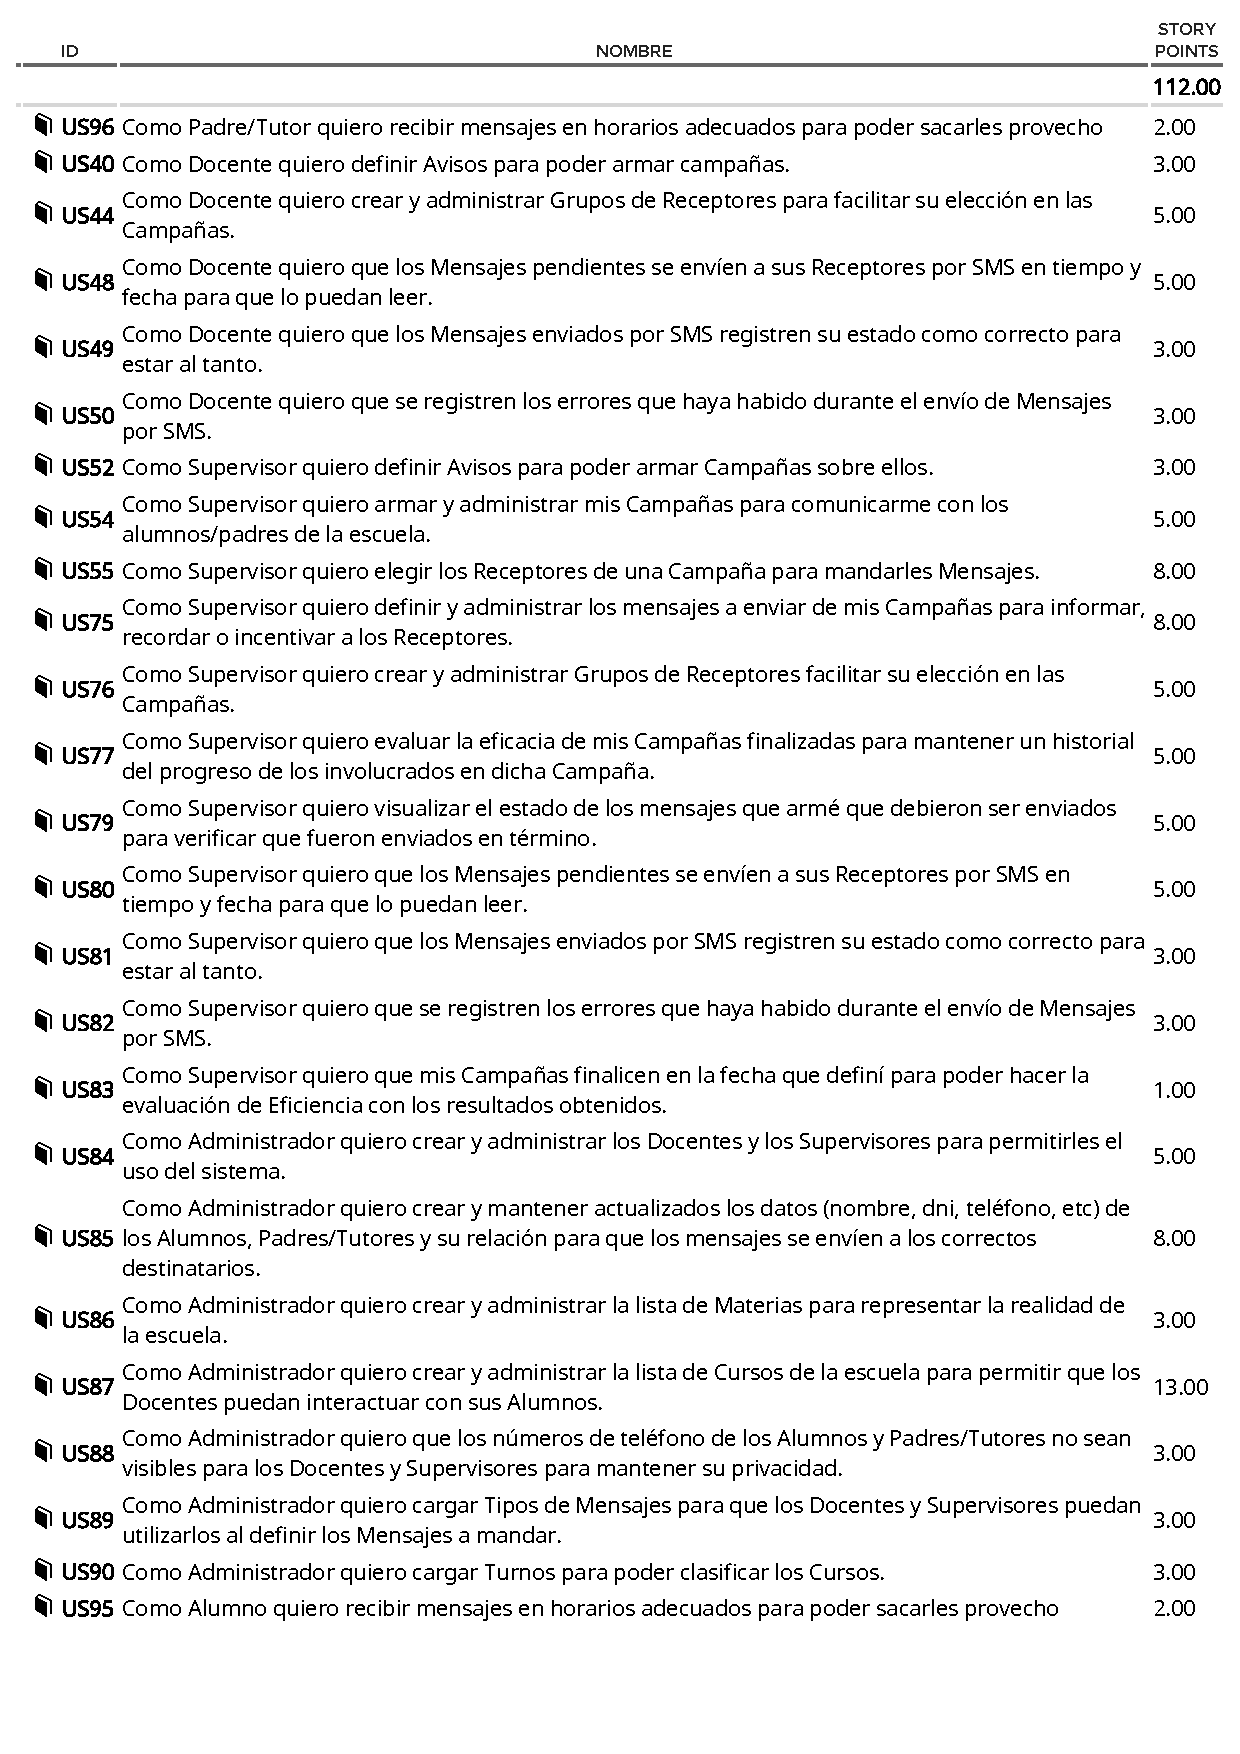
\includepdf[pages={1}]{diag/product_backlog.pdf}
	
	\invisiblesubsection{Sprint Backlog}
	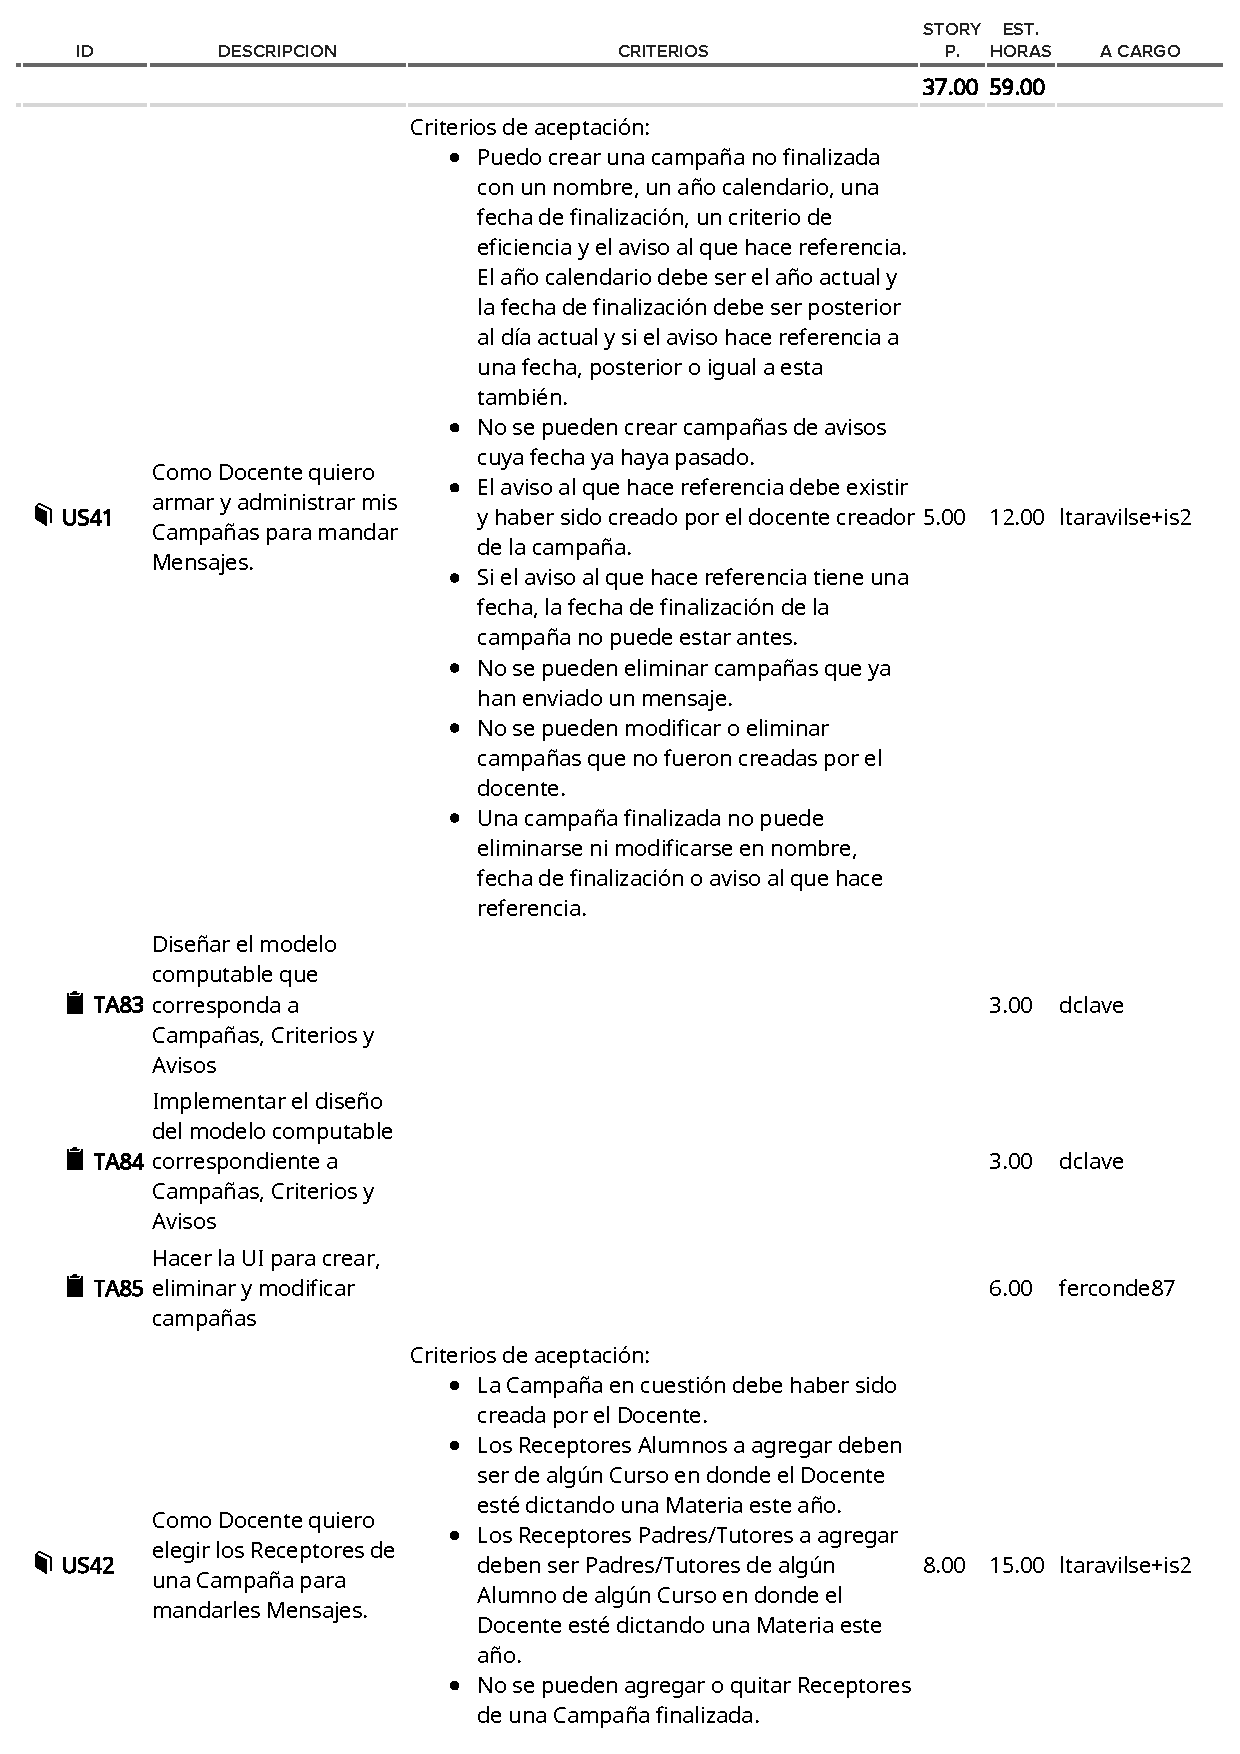
\includepdf[pages={-}]{diag/sprint.pdf}
	
\section{Seguimiento del Progreso}
	\par Como al inicio del sprint estuvimos esperando la devoluc\'on de las User Stories, no empezamos con el Dise\~no ni implementaci\'on hasta dos semanas antes de la entrega. El dise\~no se fue haciendo y rehaciendo a lo largo de las dos \'ultimas semanas, a partir de las varias consultas que hicimos sobre lo que hab\'ia que dise\~nar, y qu\'e no hac\'ia falta hacer. Por este motivo hubo muy poco avance en las tareas de implementaci\'on hasta tarde.
	\par Entrada la \'ultima semana, con un dise\~no que nos cerraba, fuimos codeando las clases del mismo, completando las tareas del sprint relacionadas a la implementaci\'on.
	\par Finalmente, el d\'ia 11/05 se testearon a mano y se dieron por aprobadas las implementaciones, completando as\'i las User Stories pertinentes.
	
	\subsection{Iteration Burndown}
	\insertfigscaled{diag/iteration_burndown}{1.0\textwidth}
	
\section{Ejecuci\'on de la Demo}
	\par La Demo funciona con Python3. Para correrlo ir al directorio ./src/ y correr el script main.py.
	
\section{Retrospectiva}
	\par Para una pr\'oxima iteraci\'on habr\'ia que haber empezado el dise\~no antes de la Reuni\'on con el Product Owner. De esta forma, de haber cambios en las stories que impacten en el dise\~no, habr\'ia que modificar algo ya hecho, en vez de hacerlo de cero.
	\par Algunos de los motivos del desv\'io tienen que ver con una cuesti\'on de tiempo. Algunos de nosotros pensamos que es mejor trabajar en algo N horas seguidas un d\'ia que dividir N en varios d\'ias, y los fines de semana suele haber el tiempo necesario para eso.
	\par Otro motivo del desv\'io es el constante cambio del Dise\~no. Hasta la \'ultima clase de consultas no tuvimos muy en claro que hab\'ia cosas que lo complejizaban y que no hab\'ia que hacer.

\section{Dise\~no OO y Justificaci\'on}
	\subsection{Dise\~no final}
		\par Los Alumnos, Responsables(Padres/Tutores), Docentes y Supervisores existen por s\'i mismos. A los Alumos y Responsables nos interesa verlos como Receptores que tienen tel\'efono y un nombre, ya que a ellos vamos a estar mand\'andoles mensajes.
		\par Las Materias, Turnos y Cursos los define alguien, y junto con los entes mencionades arriba, se registran en la Secretar\'ia. Como caso especial, para que un Alumno se registre, primero deber\'an haberse registrado sus Responsables, ya que el Alumno no se registra solo sino con sus Padres/Tutores.
		\par A un Curso pueden entrar y salir alumnos en cualquier momento del a\~no, pero por ejemplo sus materias, su turno o su nombre permanecen sin cambios.
		\par Supervisores (Director, Secretaria) y Docentes son Autoridades de la escuela, y como tales, pueden consultar en la Secretar\'ia. Un Docente no deber\'ia recibir informaci\'on sobre los cursos que no son suyos, pero un Supervisor no tiene esa restricci\'on. A su vez, s\'olo nos interesa recibir informaci\'on de un a\~no espec\'ifico (el actual).
		
		\par \phantom{a}
		\par El AdministradorDeSistema es quien maneja los Usuarios existentes, es capaz de crearlos y de validar si un username/contrase\~na es v\'alido para alguno.
		\par El Usuario es alguien que puede manipular sus Avisos, Grupos y Campa\~nas. Puede haber Docentes/Supervisores sin usuarios, pero no tiene sentido que haya Usuarios sin una Autoridad asignada, por lo que la Autoridad que representa es atributo esencial del Usuario.
		\par Como cada a\~no hay nuevos cursos, y distintos Alumnos y Padres/Tutores a los que puede acceder la Autoridad del Usuario, los Grupos son agrupaciones de Receptores restringidas a un a\~no.
		\par Un Aviso consiste en qu\'e es lo que se quiere avisar (un texto) y una fecha de evento, o de p\'erdida de inter\'es en el mismo. Por ejemplo: "`Examen de Historia"' con fecha 10/05/2015; "`No correr en los pasillos"' con fecha "`10/12/2015"' (fin de las clases).
		
		\par \phantom{a}
		\par Una Campa\~na trata de informar a los Alumnos o Padres/Tutores sobre un Aviso. Tiene un Criterio, que se define como una pregunta, y varios estados (Pendiente, Finalizada, Evaluada). Posee una fecha l\'imite propia, que debe ser igual o superior a la del Aviso, y que permite, por ejemplo, enviar un mensaje cuando est\'en corregidos los ex\'amenes (d\'ias despu\'es de que el Aviso "`Examen de Historia"' haya caducado).
		\par Para evaluarse una Campa\~na, \'esta debe haberse finalizado, por lo que el d\'ia de la fecha debe ser posterior a su fecha l\`imite. Una Evaluaci\'on consiste en una puntuaci\'on del 0 al 100 (eficiencia) y la fecha en que se evalu\'o.
		\par Las Campa\~nas pueden tener Mensajes. Es importante conocer el texto del mensaje, el tipo (Anuncio, Recordatorio, etc), la campa\~na a la que pertenece y la fecha en que quiere enviar. 
		\par El Mensaje puede estar en tres estados: Programado (no se mand\'o nada), ParcialmenteEnviado (se mand\'o a alguien) y Enviado (se mand\'o a todos). Dependiendo del estado puede removerse de la Campa\~na.
		\par Los "`mensajes enviados"' y "`parcialmente enviados"' tienen un conjunto de Confirmaciones. Estas Confirmaciones consisten en el Mensaje, a qui\'en se lo envi\'o/trat\'o de enviar, la fecha del env\'io/intento y, si hubo error durante el env\'io, qu\'e error.
		
		\par \phantom{a}
		\par Para mandar un mensaje, se necesita un Mensajero. La Mensajer\'ia lo conoce, y se encarga de buscar los mensajes pendientes para enviarlos. A un Mensaje, se le pide "`enviarse si est\'a pendiente"' y se le adjunta el Mensajero. En caso de estar pendiente, para cada Receptor no enviado, el Mensaje se encarga de pedirle al Mensajero que se lo env\'ie. \'Este le responde con una Confirmacion, que tendr\'a el resultado del env\'io/intento.
		\par La Mensajer\'ia tambi\'en registra los Tipos de Mensajes disponibles, y se le pueden consultar cu\'ales tiene registrados.
		
		\par \phantom{a}
		\par Un reloj es una entidad que mide el tiempo. En nuestro caso, se puede ajustar en fecha y tiempo. El Reloj conoce Notificadores, que pueden agregarse y sacarse en todo momento. Ante un ajuste del Reloj, se notifican a todos sus Notificadores para que act\'uen en consecuencia. Este Observer permite que, ante un cambi\'o en la fecha, los procesos sensibles al paso del tiempo como la Mensajer\'ia se ejecuten (en este caso, enviar\'a los mensajes pendientes respecto a la nueva fecha).
		\par A su vez, otro proceso y Notificador que depende del tiempo es el Finalizador de Campa\~nas, que consiste en finalizar las Campa\~nas pendientes con fecha l\'imite igual o 
previa a la fecha que indique el Reloj.

	\subsection{Dise\~nos descartados}
		\par Los dise\~nos previos inclu\'ian mucho uso de Visitor, Factory y Proxy. Pens\'abamos que era necesaria la persistencia de los objetos, por lo que hab\'ian varios "`Managers"' que se encargaban de buscar los datos de un ente, crearlo, wrappearlo en un Proxy y devolverlo. Durante la \'ultima consulta con el Tutor se aclar\'o que esto no era necesario y el Dise\~no se simplifico much\'isimo en consecuencia.
	
	%Dise�o OO y justificaci�n. Se deben entregar todos los diagramas que crean necesarios
%para explicar correctamente el funcionamiento de su dise�o. Esto incluye diagramas de objetos,
%clases y colaboraci�n (junto a sus escenarios). Todas las decisiones deben estar
%correctamente justificadas, as� como las alternativas planteadas y finalmente descartadas. Para
%la resoluci�n de esta parte del TP se busca fuertemente que utilicen los conceptos vistos
%durante el curso y se corregir� en consecuencia.

	\subsection{Diagrama de Clases}
		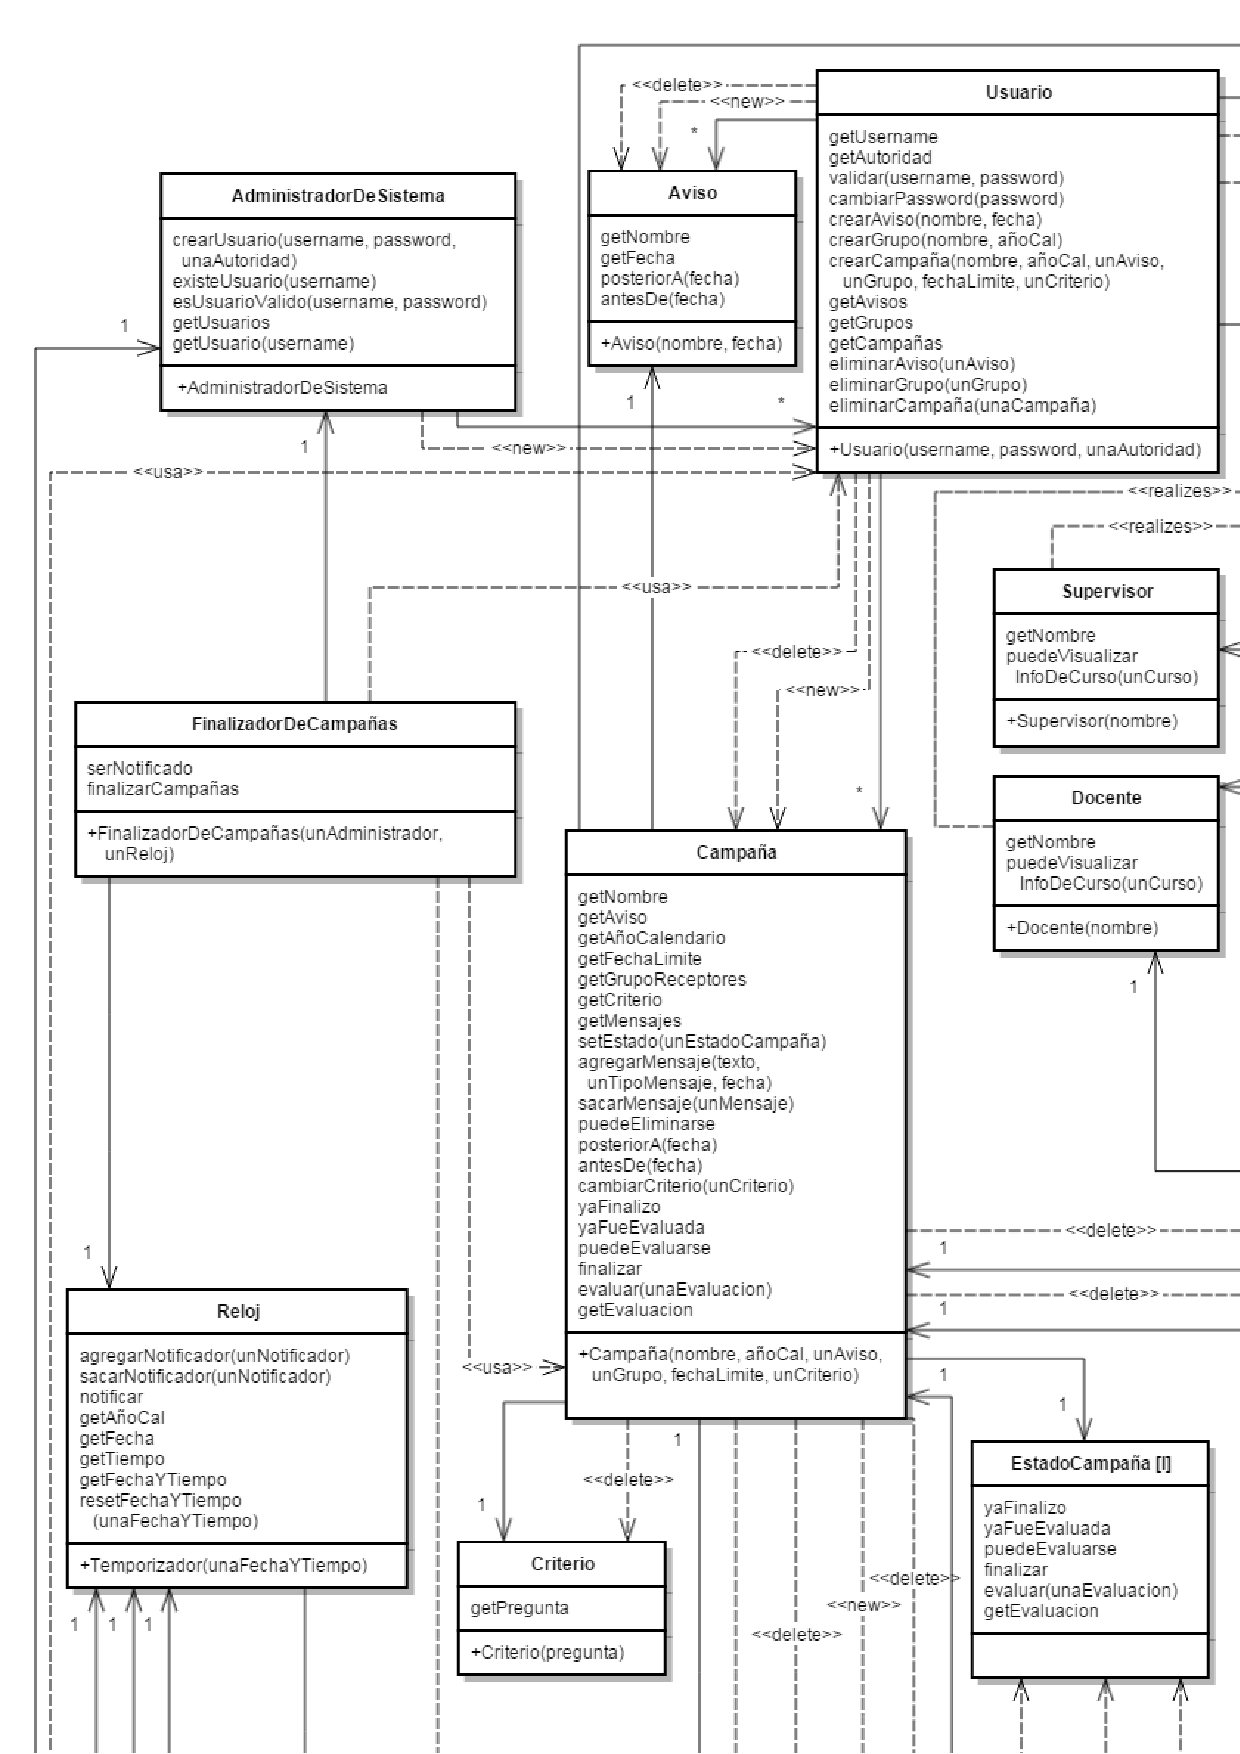
\includepdf[pages={1,3,2,4}]{diag/clases.pdf}
		
	\subsection{Diagrama de Objetos y Secuencia para el Escenario 1}
	\par En un mundo paralelo, Severus Snape quiere armar una campa\~na del aviso "`Examen de DADA"' para los alumnos de "`Gryffindor 2015"'.
	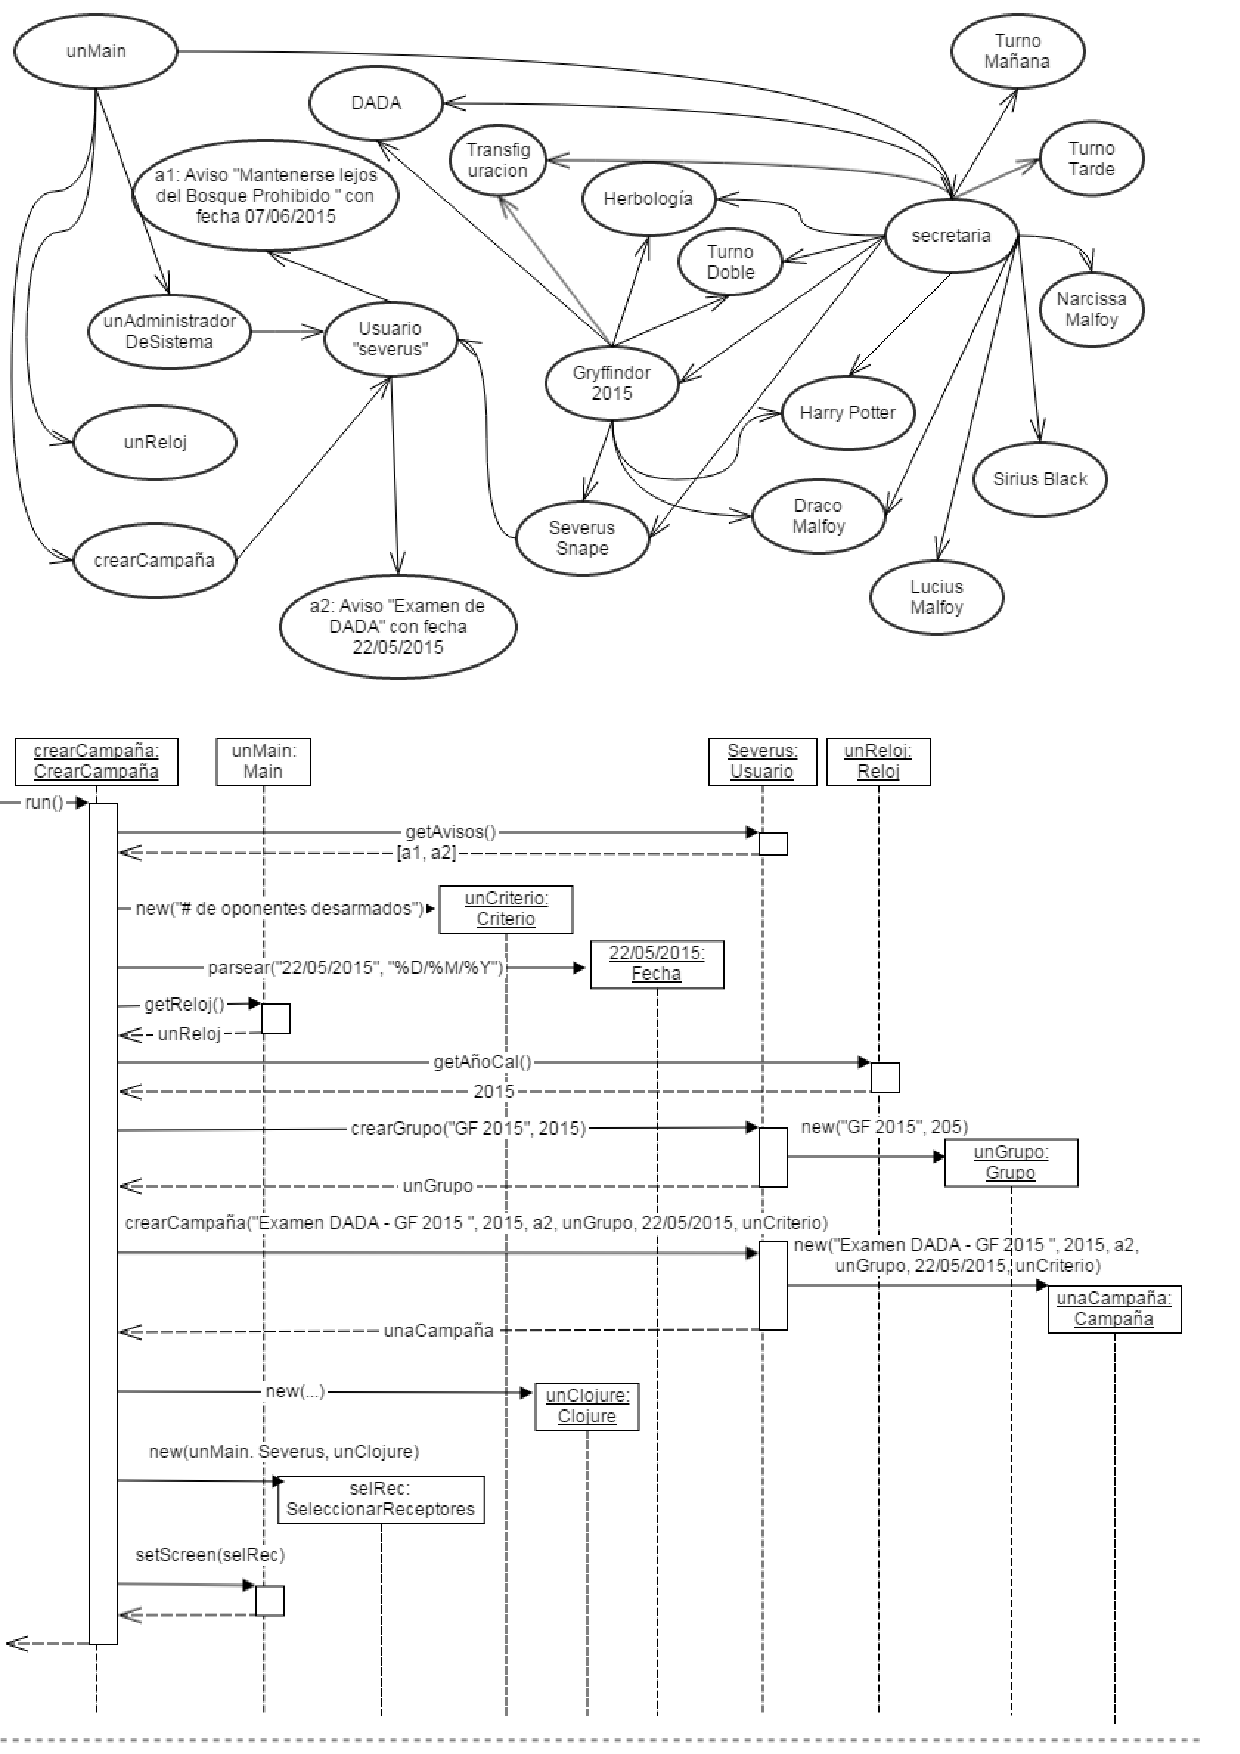
\includepdf[pages={-}]{diag/escenario1.pdf}
	
	\subsection{Diagrama de Objetos y Secuencia para el Escenario 2}
	\par Severus Snape ahora quiere preparar un mensaje de tipo "`Anuncio"' para ser enviado el 10/05/2015 utilizando la campa\~na que reci\'en cre\'o.
	\par Con el paso del tiempo, el mensaje se env\'ia a Harry Potter y a Draco Malfoy.
	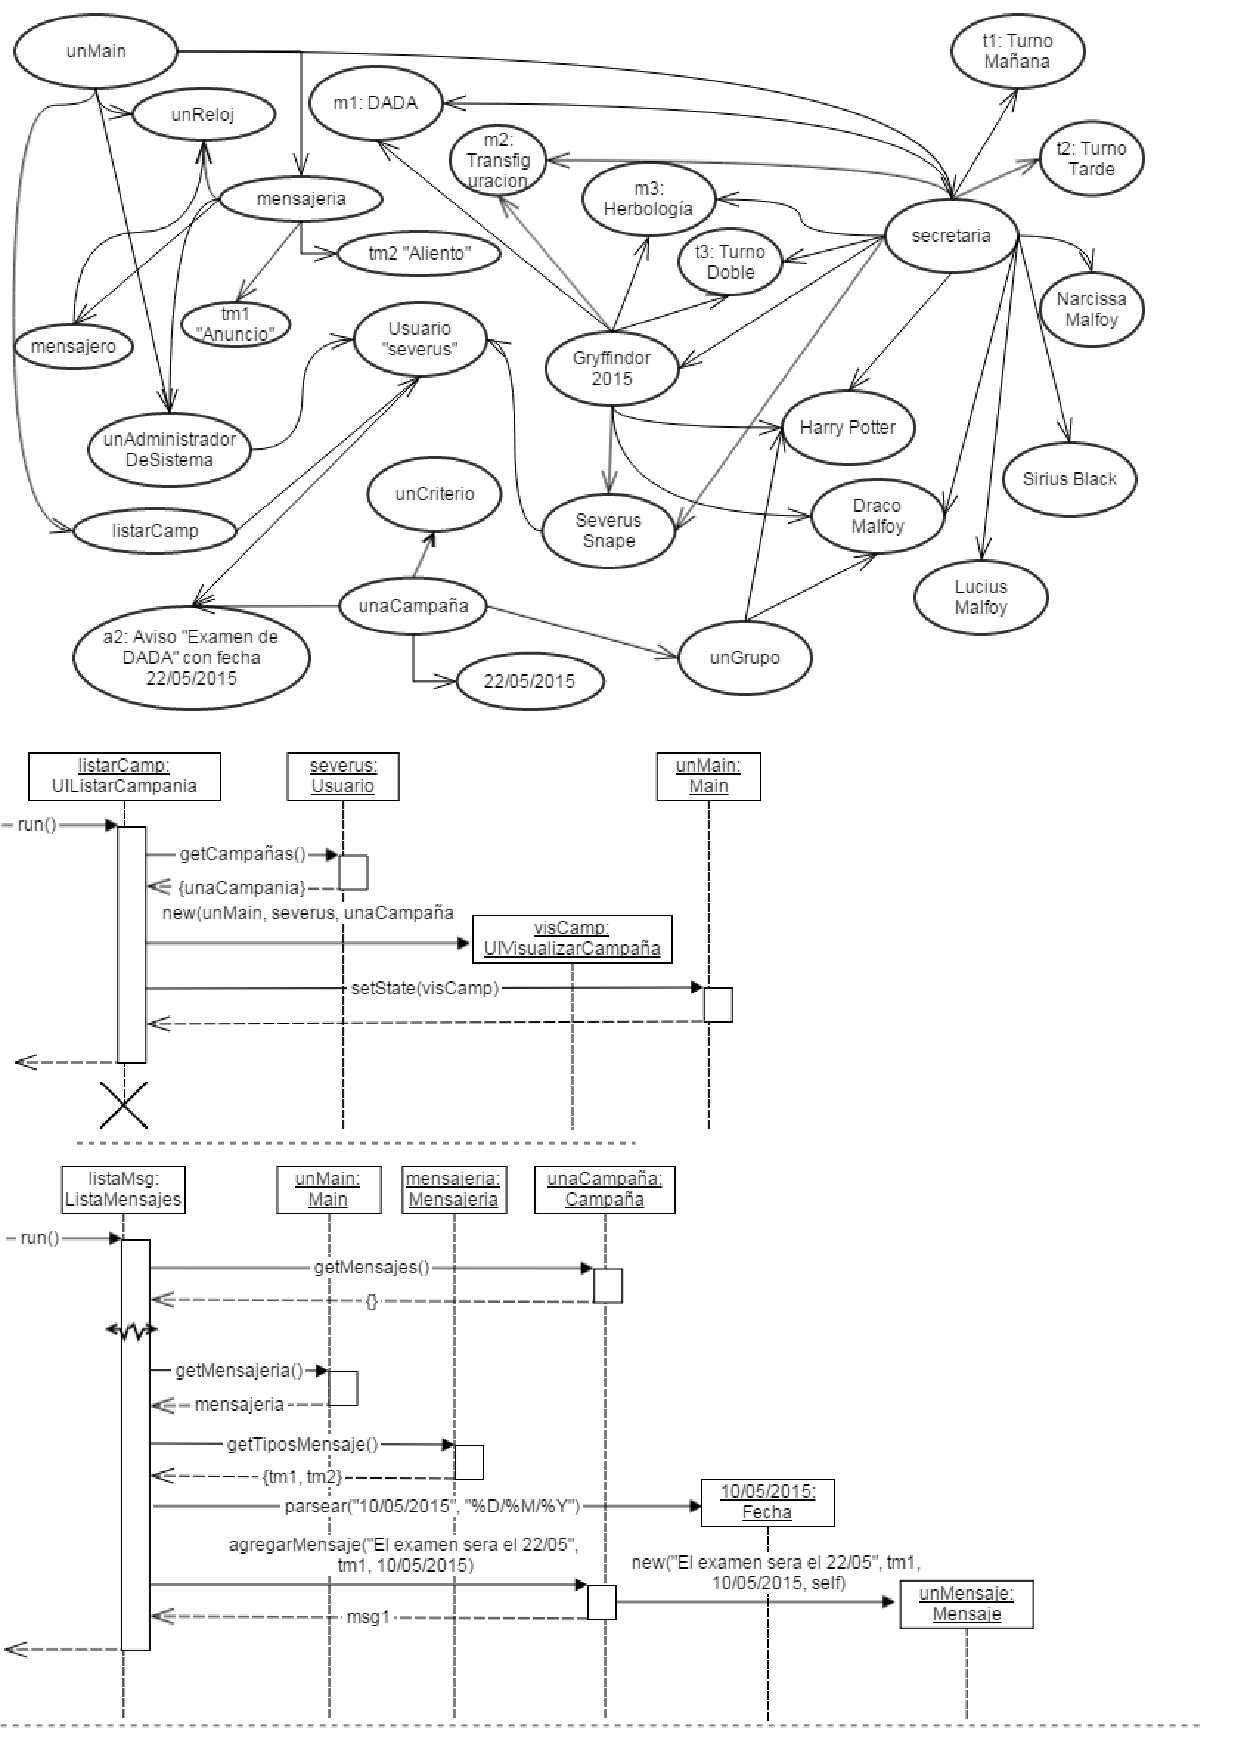
\includepdf[pages={-}]{diag/escenario2.pdf}


\end{document}
